\documentclass[UTF8]{ctexart}
\usepackage{amsmath}
\usepackage{geometry}
\usepackage{diagbox}
\usepackage{bm}
\usepackage{gensymb}
\usepackage{graphicx}
\usepackage{titlesec}
\usepackage{wrapfig}
\geometry{a4paper,scale=0.8}
\title{2019年电磁场与波期末试题}
\author{Deschain}
\titlespacing*{\section}
{0pt}{0pt}{0pt}
\titlespacing*{\subsection}
{0pt}{0pt}{0pt}
\titlespacing*{\paragraph}
{0pt}{0pt}{0pt}
\titlespacing*{\subparagraph}
{0pt}{0pt}{0pt}
\begin{document}
\maketitle
\section{}
\begin{wrapfigure}{r}{4cm}
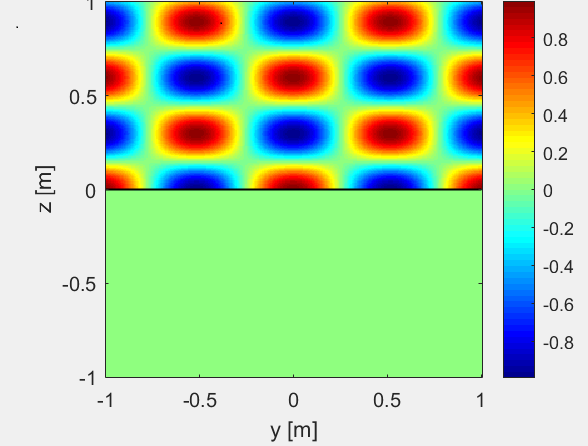
\includegraphics[width=4cm]{2019-1.png}
\end{wrapfigure}
\paragraph{}
已知由理想导体组成的平板波导,某场的X分量大小如下图所示,场的频率为260MHz,场的传播方向为Y轴正方向。
\subsection{}
\paragraph{}
判断是TM波还是TE波?为什么?
\subparagraph{解答}
TM波。因为切向场在导体边界上存在,所以是磁场。
\subsection{}
\paragraph{}
计算波导中介质的相对介电常数。
\subparagraph{解答}
\begin{equation*}
\begin{aligned}
&\lambda_z=0.6m,k_z=\frac{2\pi}{\lambda_z}\\
&\lambda_y=1m,k_y=\frac{2\pi}{\lambda_y}\\
&k=\sqrt{k_z^2 + k_y^2},k^2=\omega^2\mu \varepsilon=\omega^2\mu_0\varepsilon_r\varepsilon_0\\
&\varepsilon_r=\frac{k^2}{\omega^2\mu_0\varepsilon_0}=5.03
\end{aligned}
\end{equation*}
\subsection{}
\paragraph{}
写出电场与磁场各个方向的分量表达式(要写出传播项、时谐项)。
\subparagraph{解答}
\begin{equation*}
\begin{aligned}
&\vec{H}=\hat xAcos(k_zz)e^{j(\omega t-k_yy)}\\
&\vec{E}=\hat zBcos(k_zz)e^{j(\omega t-k_yy)} +\hat yCjsin(k_zz)e^{j(\omega t-k_yy)}
\end{aligned}
\end{equation*}
\subsection{}
\paragraph{}
画出Y方向半个周期的电场和磁场的三维场结构。
\begin{figure}[htbp]
\centering
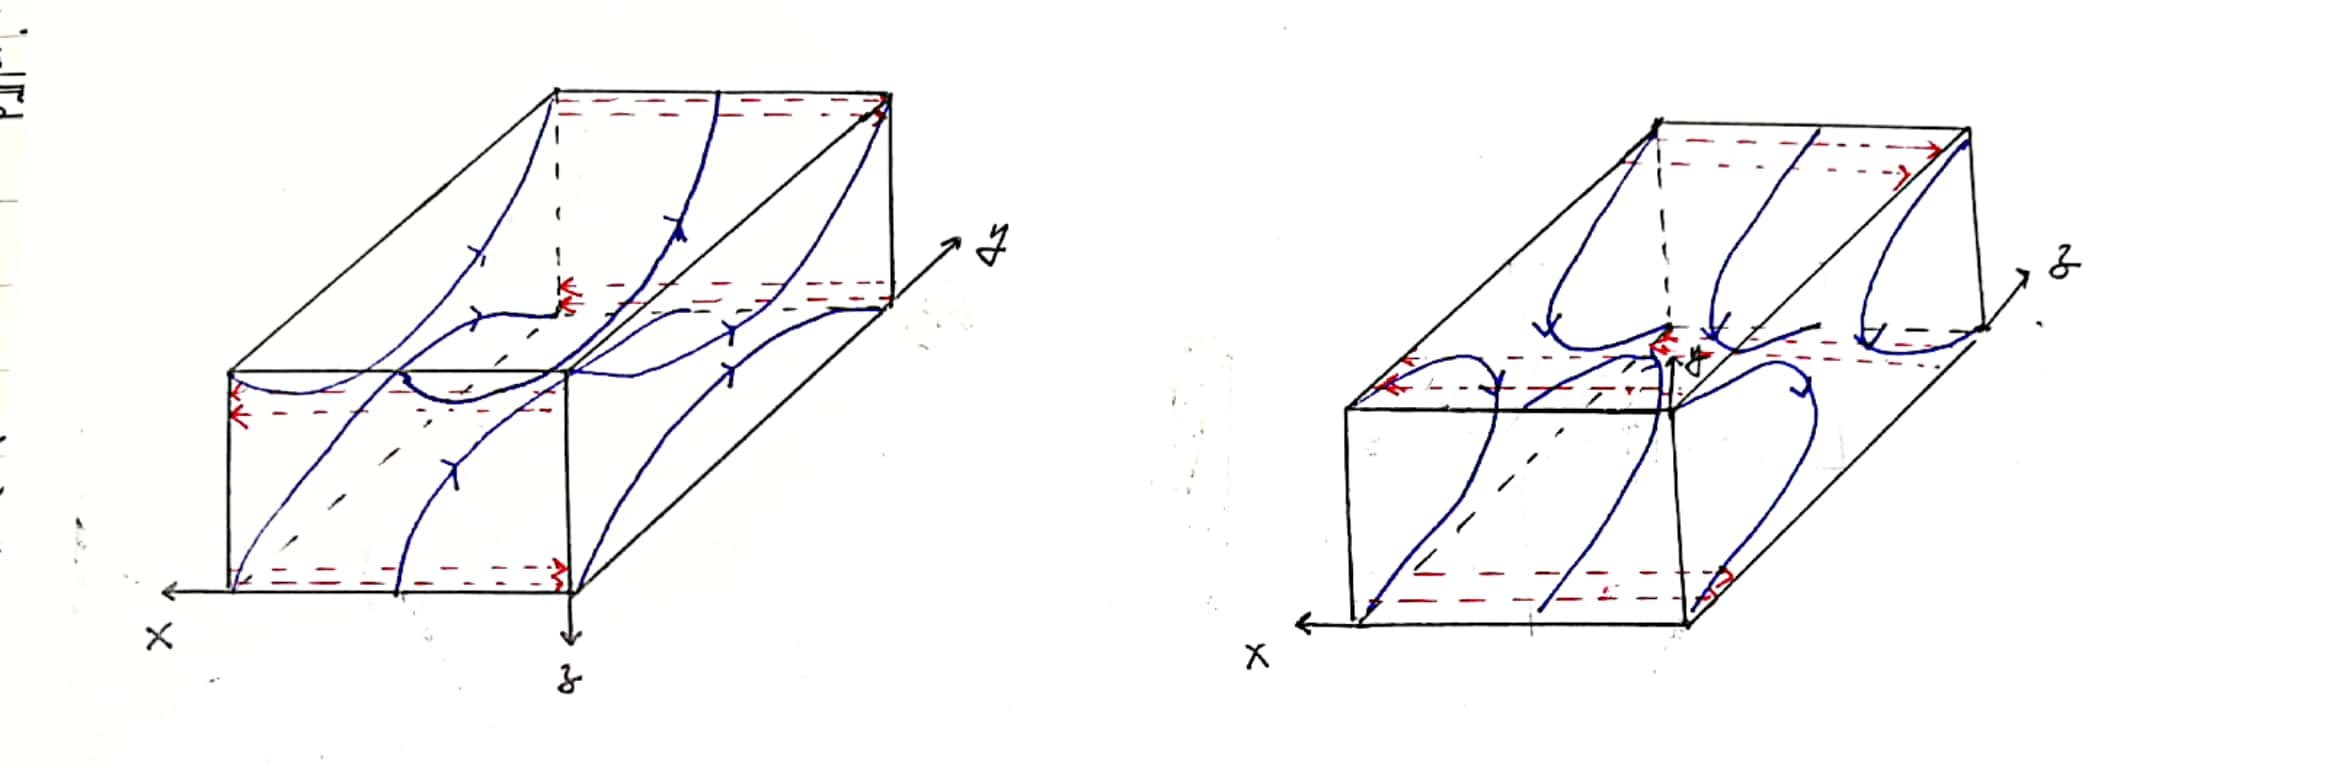
\includegraphics[width=14cm,height=4cm]{2019-2.jpg}
\end{figure}
\section{}
\subsection{}
\paragraph{静电场}
在原点附近放置一定数量电荷,使之在X轴正向远离原点处产生的电场总平行于方向$\vec A=\hat\theta+\hat\phi$。写出电荷的位置,相对电荷大小。
\subparagraph{解答}
(0,-d,0):+q\\
(0,d,0):-q\\
(0,0,d):+q\\
(0,0,d):-q\\
\subsection{}
\paragraph{时变电磁场}
在原点附近放置一定数量辐射源,使之在X轴正方向远离原点处产生的电场总平行于方向$\vec A=\hat\theta+\hat\phi$。如果可以,写出辐射源的情况;如果不可以,请写出理由。
\subparagraph{解答}
在z轴上沿z轴负向放置一个辐射电偶极子,在y轴上沿y轴负向放置一个辐射电偶极子,两者等大,等相位。
\subsection{}
\paragraph{}
写出X轴上右旋圆极化波的球坐标表示。
\subparagraph{解答}
\[ \vec E=(\hat \phi-j\hat \theta)e^{j(\omega t-kr)}\]
\subsection{}
\paragraph{时变电磁场}
在原点附近放置一定数量辐射源,使之在$\theta =45\degree$的等值平面上远离原点处产生的电场总平行于方向$\vec A=\hat\theta + \hat\phi$,如果可以,写出辐射源的情况;如果不可以,写出理由。
\subparagraph{解答}
沿y轴正向放置一个电偶极子和一个磁偶极子,两者在等值面上产生的电场大小相同,相位相同。
\section{}
\paragraph{}
已知有一圆柱形静电场区域,满足如下边界条件:$Z=0$时,$\varphi=0$,$Z=30$时,$\varphi=5V+g(\rho,\varphi)$,$\rho=10$时,$\varphi=5V+h(z,\phi)$。
\subsection{}
\paragraph{}
写出电势表达式通解,并说明理由。
\subparagraph{解答}
\[\varphi = \varphi_1 + \varphi_2\]
$\varphi_1$是“$Z=30$时,$\varphi=5V+g(\rho,\varphi)$,其余为0”对应的电势。
$\varphi_2$是“$\rho=10$时,$\varphi=5V+h(z,\phi)$,其余为0”对应的电势。
\[\varphi_1=\sum_{n=0}^{}\sum_{i=1}^{}[A_{ni}sin(n\phi)]+B_{ni}cos(n\phi)]J_n(k_{zi}^{(n)}\rho)sh(k_{zi}^{(n)}z)\quad n=0,1,2,3\cdots\]
\[\varphi_2=\sum_{m=1}^{}\sum_{k=1}^{}[A_{mk}sin(m\phi)+B_{mk}cos(m\phi)]sin(\frac{k\pi}{b}z)I_m(\frac{k\pi}{b}z)\]
\[\varphi=\varphi_1+\varphi_2\]
\subsection{}
\paragraph{}
画出$g=0$,$h=0$时$X=0$平面上的电场线和等势面。
\begin{figure}[htbp]
\centering
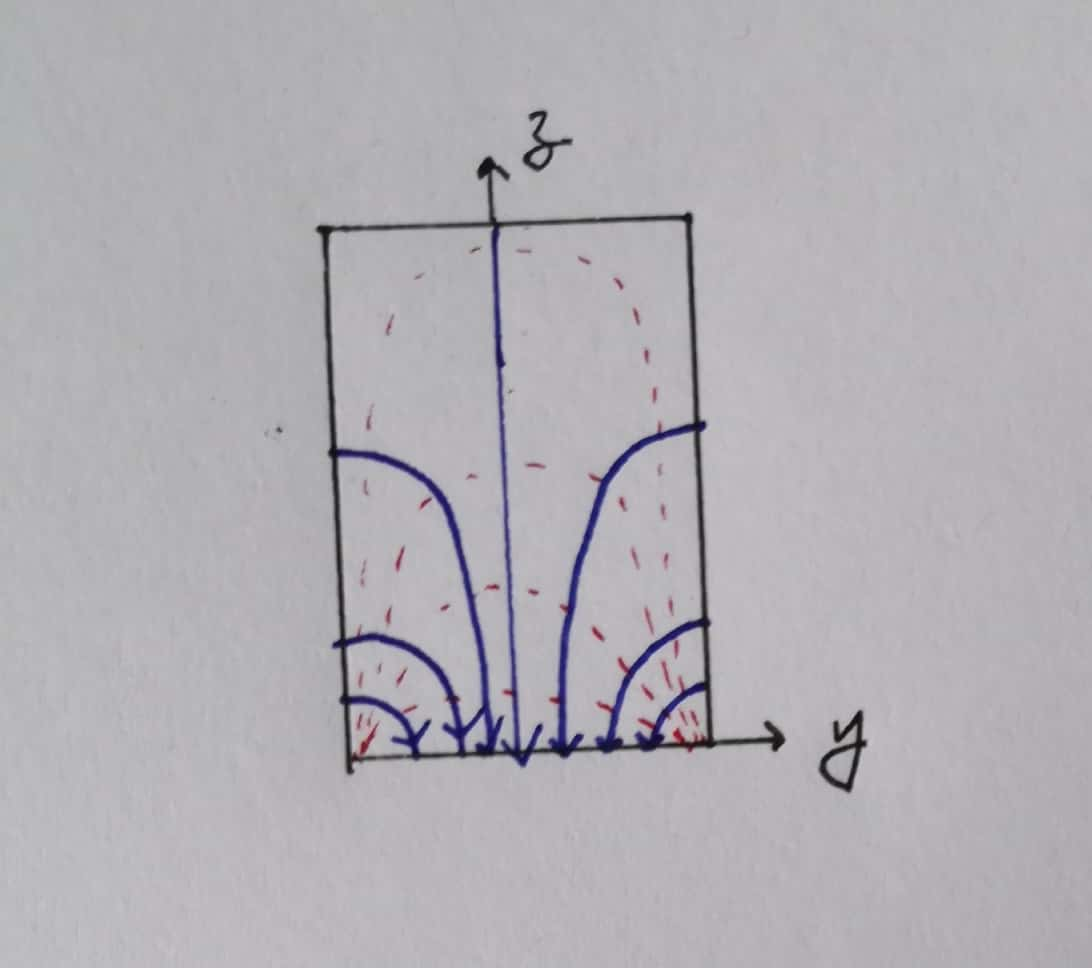
\includegraphics[width=3.5cm,height=4cm]{2019-3.jpg}
\end{figure}
\section{}
\paragraph{}
已知有谐振腔,5个面是磁壁,1个面是电壁(右面),尺寸为$20mm\times 30mm\times30mm$ (XYZ)。
\begin{wrapfigure}{r}{4cm}
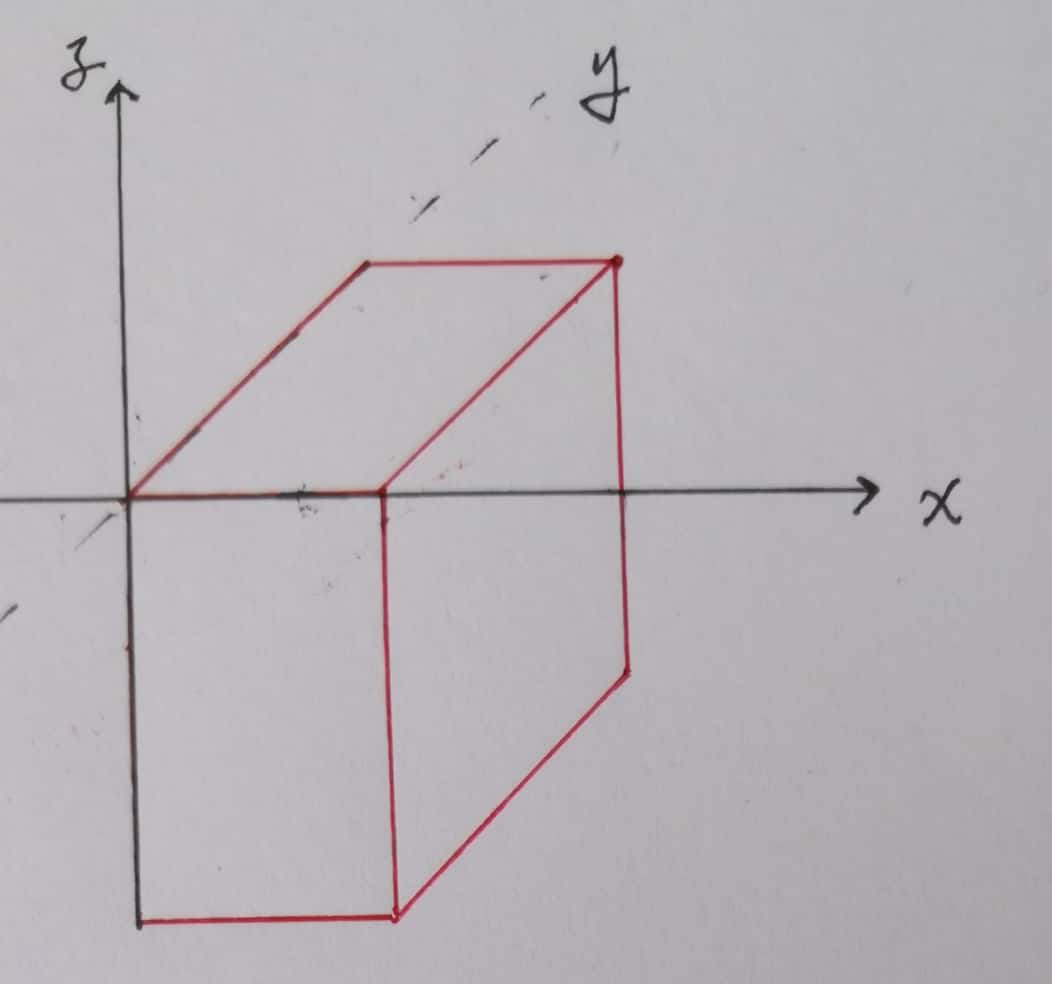
\includegraphics[width=4cm]{2019-4.jpg}
\end{wrapfigure}
\subsection{}
\paragraph{}
写出这一谐振腔最低两个模态的频率。
\subparagraph{解答}
在110模式与101模式下,频率为6.25GHz。
\subsection{}
\paragraph{}
分别写出最低两个模态各个方向的场分量。
\subparagraph{解答}
在110模式下:
\begin{equation*}
\begin{aligned}
&E_x=jE_1sin(\frac{\pi x}{2a})cos(\frac{\pi y}{b})\\
&E_y=jE_2cos(\frac{\pi x}{2a})sin(\frac{\pi y}{b})\\
&H_z=H_1sin(\frac{\pi x}{2a})sin(\frac{\pi y}{b})
\end{aligned}
\end{equation*}
在101模式下;
\begin{equation*}
\begin{aligned}
&E_x=E_3sin(\frac{\pi x}{2a})cos(\frac{\pi z}{l})\\
&E_z=E_4cos(\frac{\pi x}{2a})sin(\frac{\pi z}{l})\\
&H_y=H_2sin(\frac{\pi x}{2a})sin(\frac{\pi z}{l})
\end{aligned}
\end{equation*} 
\subsection{}
\paragraph{}
画出最低两个模态中H场有Y方向分量的模态的电场与磁场的三维场结构。
\begin{figure}[htbp]
\centering
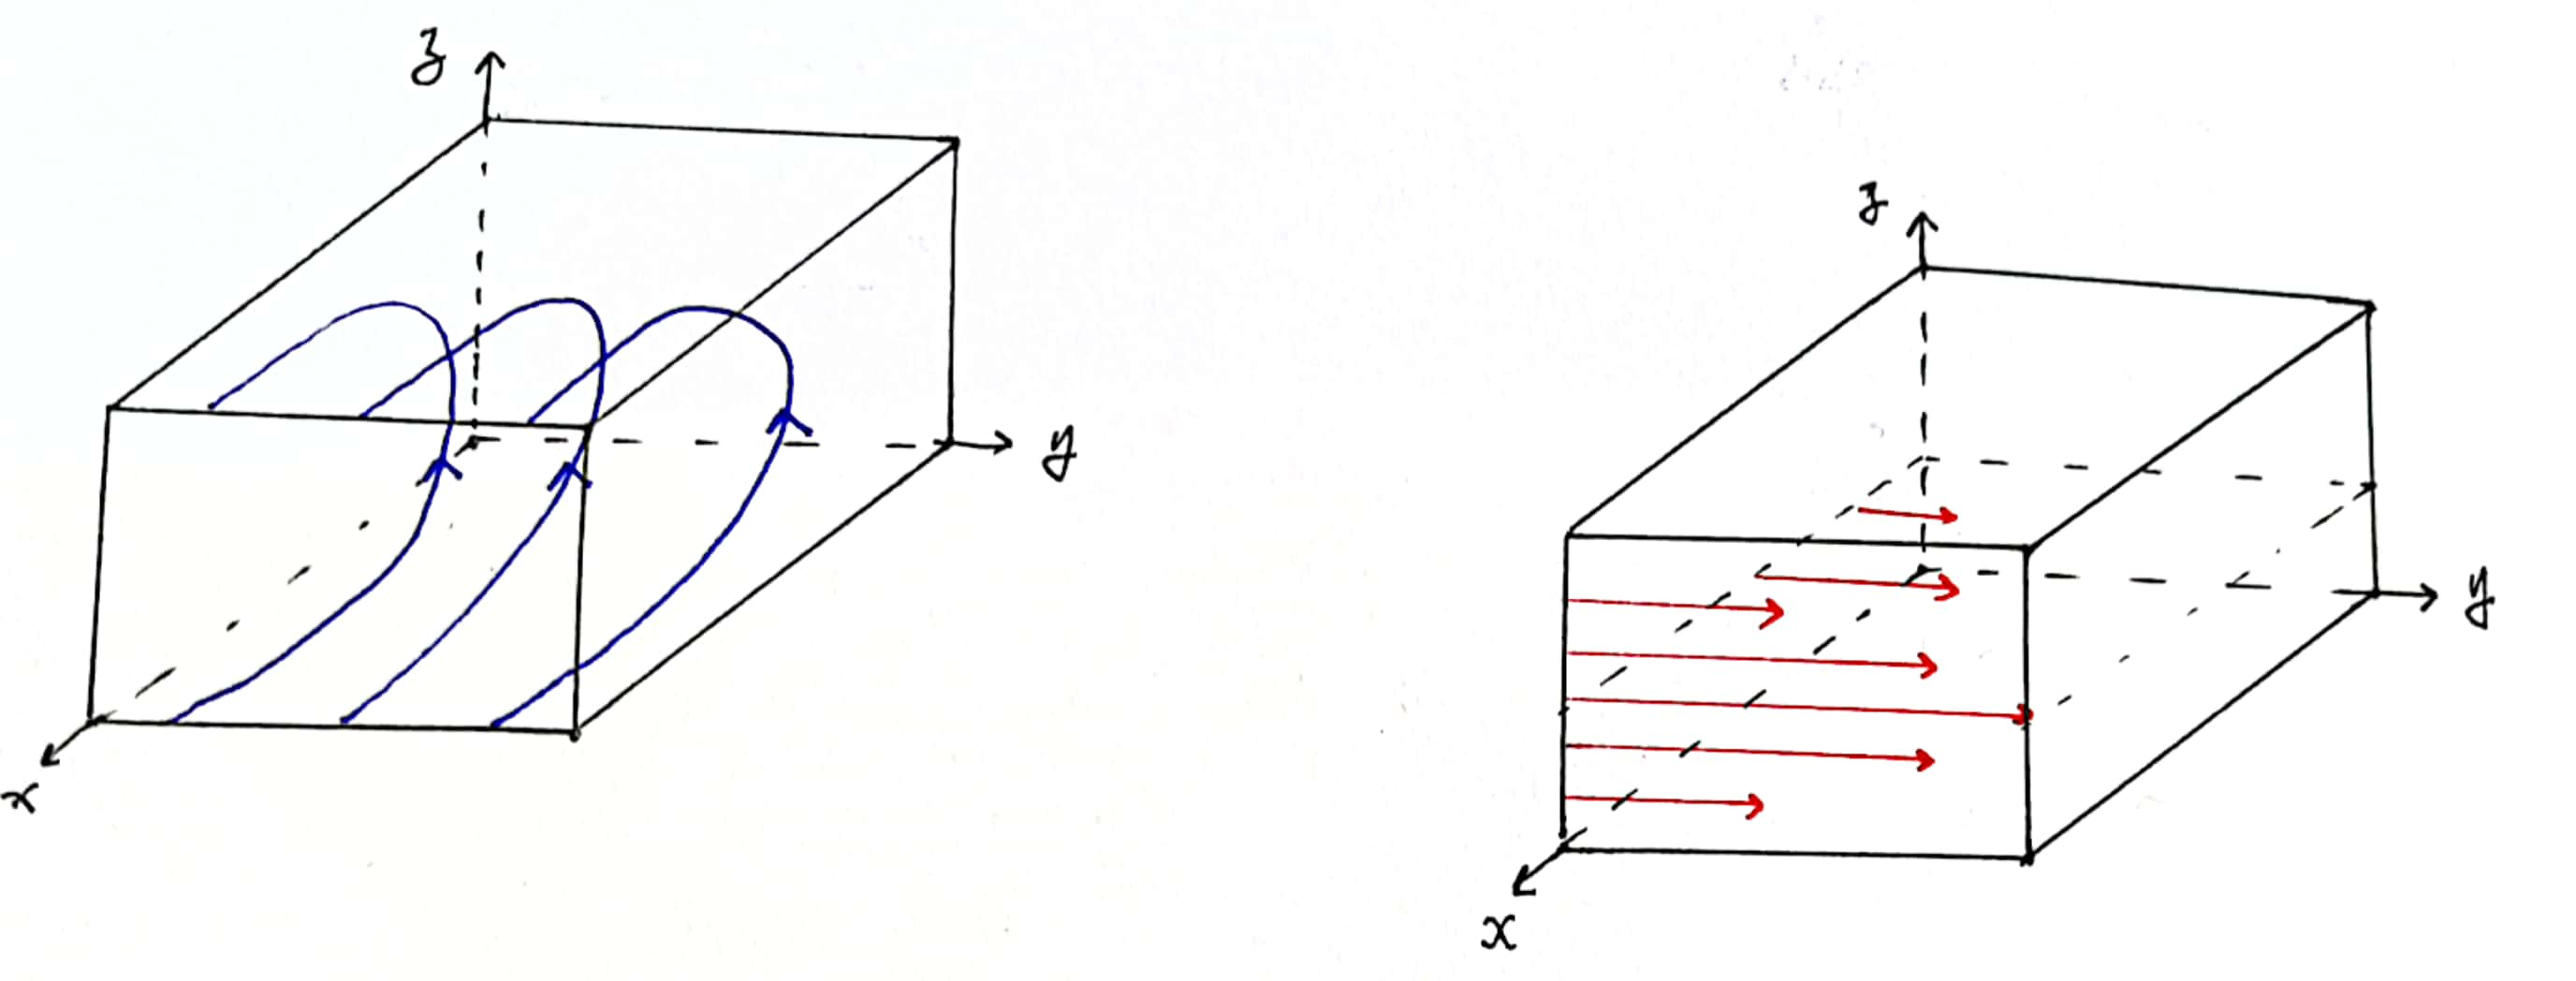
\includegraphics[width=14cm,height=4cm]{2019-5.jpg}
\end{figure}
\paragraph{}
是101模式。
\end{document}